\title{LEZIONE 5 31/03/2020}\newline
\textbf{link} \href{https://web.microsoftstream.com/video/acc276af-8db7-418e-bd82-ab22809fb6ac}{clicca qui}
\section{Cinematica del manovellismo ordinario}
\subsection{Introduzione}
[immagine dagli appunti del prof]
\begin{center}
    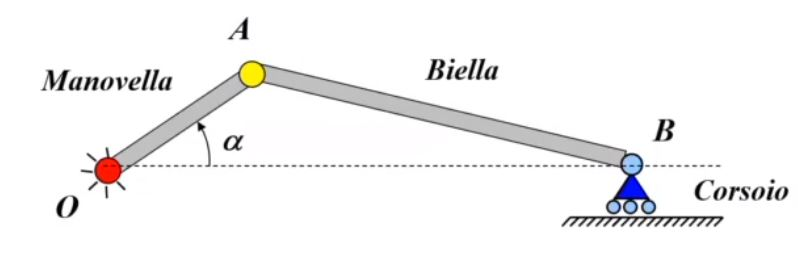
\includegraphics[height=3cm]{../lezione5/img1.JPG}
\end{center}
Il \textbf{manovellismo oridnario} è un sistema costituito da tre corpi: un corpo rotante detto \textbf{manovella} (rosso), un corpo che effettua una traslazione che viene chiamato \textbf{corsoio} (giallo) e, infine, un elemento chiamato \textbf{biella} (marrona).\newline
\newline
il punto $A$ prende il nome di \textbf{bottone di manovella} e il punto $B$ prende il nome di \textbf{piede di biella}.\newline
\newline
Il manovellismo ordinario serve per trasformare un moto rotatorio in un moto traslatorio alternato (o viceversa).\newline
\newline
Perchè sia possibile che la manovella possa compiere una rotazione a 360 gradi è necessario che il raggio della manovella sia minore del raggio della biella.\newline
\newline
Questo meccanismo è una \textbf{catena chiusa}, con un unico grado di libertà ($\alpha$).\newline
\newline
Esistono due tipi di manovellismi:
\begin{itemize}
    \item \textbf{manovellismo ordinario centrato}: il moto del punto $B$ è un moto traslatorio alternato lungo un asse che passa per il punto $O$.
    \item \textbf{manovellismo ordinario deviato}: se non è centrato.
\end{itemize}
In questo corso studieremo il manovelismo ordinario centrato.
\subsection{Posizione del manovellismo ordinario centrato}
Noto $\alpha$, $\dot{\alpha}$, $\ddot{\alpha}$, con $\dot{\alpha} = \omega = costante$, studiamo la posizione del punto $B$.\newline
\newline
Per farlo usiamo l'\textbf{equazione di chiusura}, cioè l'equazione che descrive il poligono chiuso composto da manovella, biella e telaio:\newline
[immagine dagli appunti del prof]
\begin{center}
    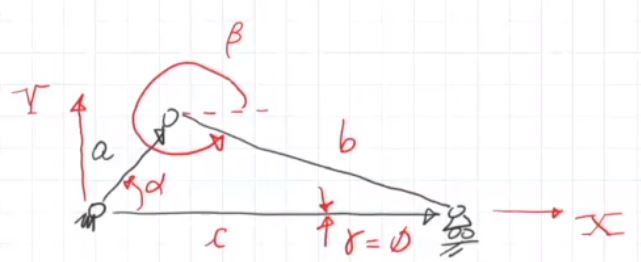
\includegraphics[height=3cm]{../lezione5/img2.JPG}
\end{center}
\[
    (A-O) + (B-A) = (B-O)
\]
\[
    a e^{i \alpha} + b e^{i \beta} = c e^{i \gamma}
\]
Imponiamo il vincolo che il la manovella sia minore della biella e cioè che:
\[
    \lambda = \frac{a}{b} < 1
\]
dove $\lambda$ prende il nome di \textbf{rapporto caratteristico del manovellismo}.\newline
Un altro vincolo da imporre è che l'angolo $\beta$ sia:
\[
    \beta \in [90, 90]
\]
Infine, $\gamma$ fa parte del telaio immobile e quindi è sempre nullo.\newline
\newline
Dunque:
\[
    a e^{i \alpha} + b e^{i \beta} = c e^{i \gamma} = c
\]
Separando parte reale e immaginaria ottengo:
\[
    \begin{cases}
        a cos(\alpha) + b cos(\beta) = c\\
        a sin(\alpha) + b sin(\beta) = 0
    \end{cases}
\]
Dalla seconda equazione ottengo che $sin(\beta) = \frac{a}{b} sin(\alpha) = \lambda sin( \alpha)$ e considerando che $sin^2(\beta) + cos^{2} (\beta) = 1$, allora $cos(\beta) = \sqrt{1-\lambda^2 sin^2(\alpha)}$.
\[
    \begin{cases}
        c = a cos(\alpha) + b \sqrt{1- \lambda^2 sin^2(\alpha)}\\
        \beta = a sin(-\lambda sin(\alpha))
    \end{cases}
\]
Abbiamo così determinato $c(t)$ e $\beta(t)$.\newline
\newline
Analiziamo ora il caso particolare in cui $\alpha = 0$, cioè in cui $c = c_{max} = a+b$, questo punto è il punto di massima estensione e prende il nome di \textbf{punto morto esterno}.\newline
In questo punto la velocità di $B$ si annulla, mentre l'accellerazione di $B$ risulta essere massima in modulo.\newline
\newline
Al contrario si ha la velocità massima del punto $B$ circa (!) per un valore di $\alpha$ pari a $\frac{\pi}{2}$. In questo caso $c = \sqrt{b^2 - a^2}$ e $\vec{v}_B \sim v_{max}$.\newline
\newline
Se $\alpha = \pi$, la distanza $c$ sarà minima, cioè $c = c_{min} = b-a$ e questo punto prende il nome di \textbf{punto morto interno}.\newline
\newline
Il moto del corsoio è rappresentabile circa così:\newline
[immagine dagli appunti del prof]
\begin{center}
    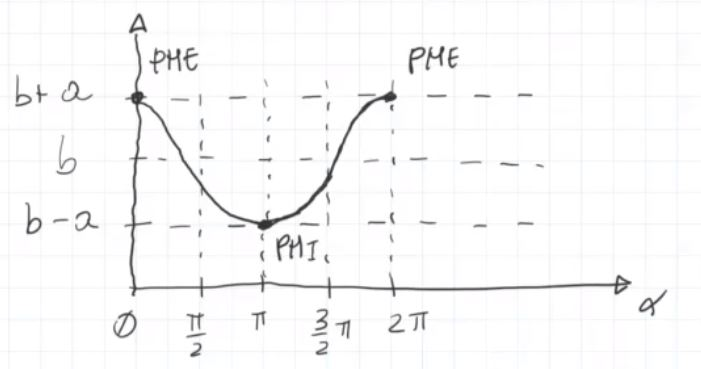
\includegraphics[height=4cm]{../lezione5/img3.JPG}
\end{center}
ed si avvicina a un modo cosinusoidale quanto più $\lambda = \frac{a}{b}$ è minore di $1$.
\subsection{Velocità del manovellismo ordinario centrato}
Derivando le equazioni di chiusura ottenute precedentemente otteniamo:
\[
    i a \dot{\alpha} e^{i \alpha} + i b \dot{\beta} e^{i \beta} = \dot{c}
\]
\[
    a \dot{\alpha} e^{i (\alpha + \frac{\pi}{2})} + b \dot{\beta} e^{i (\beta + \frac{\pi}{2})} = \dot{c}
\]
Andiamo a interpretare questi termini con il teorema dei moti relativi, per una terna mobile posizionata nel punto $A$:
\begin{itemize}
    \item velocità di trascinamento di $B$ è $\vec{v}_{tr,B} = a \dot{\alpha} e^{i (\alpha + \frac{\pi}{2})}$
    \item velocità relativa di $B$ è $\vec{v}_{rel,B} = b \dot{\beta} e^{i (\beta + \frac{\pi}{2})}$
\end{itemize}
\ \newline
Proiettiamo ora sull'asse $X$ e $Y$ l'equazione per ottenre il sistema:
\[
    \begin{cases}
        - a \dot{\alpha} sin(\alpha) - b \dot{\beta} sin(\beta) = \dot{c}\\
        a \dot{\alpha} cos(\alpha) + b \dot{\beta} cos(\beta) = 0
    \end{cases}
\]
Questo sistema è un sistema in due equazioni e in due incognite ($\dot{c}, \dot{\beta}$):
\[
    \left[\begin{matrix}
        1 & b \; sin(\beta)\\
        0 & -b \; cos(\beta)
    \end{matrix}\right] \left[\begin{matrix}
        \dot{c} \\ \dot{\beta}
    \end{matrix}\right] = \left[\begin{matrix}
        - a \dot{\alpha} sin(\alpha) \\ a \dot{\alpha} cos(\alpha)
    \end{matrix}\right]
\]
\subsubsection{Jacobiano del moto}
Il procedimento appena seguito per determinare la velocità del punto $B$ poteva essere semplificato usando il jacobiano del moto.\newline
\newline
Il \textbf{Jacobiano del moto} rappresenta la velocità di un punto di interesse ($B$) rapportato alla derivata prima della coordianta indipendente (del grado di libertà, cioè dell'angolo della manovella).
\[
    \Lambda = \frac{v_B}{\dot{\alpha}} = \frac{\dot{c}}{\dot{\alpha}} = \Lambda(\alpha) = -a [sin(\alpha)- cos(\alpha) tg(\beta)]
\]
\[
    \Lambda = \frac{\dot{c}}{\dot{\alpha}} = \frac{dc}{dt} \cdot \frac{dt}{d \alpha} = \frac{dc}{d \alpha} = \Lambda (\alpha)
\]
\[
    \dot{\alpha} = \Omega = costante \Rightarrow v_B = \Lambda (\alpha) \dot{\alpha} = \Lambda (\alpha) \Omega = \frac{dc}{d \alpha} \Omega
\]
\ \newline
Vediamo ora una rappresentazione della velocità:\newline
[immagine dagli appunti del prof]
\begin{center}
    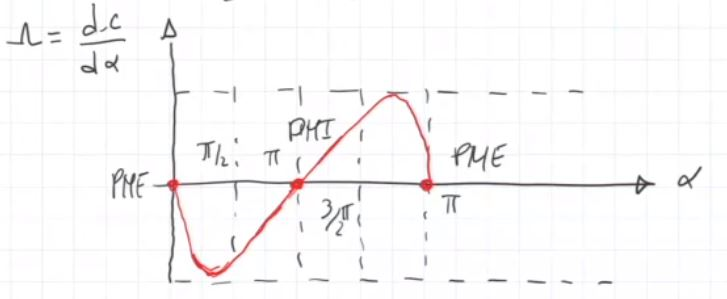
\includegraphics[height=3cm]{../lezione5/img4.JPG}
\end{center}
\subsection{Accellerazione del manovellismo ordinario centrato}
Come per la velocità, ci basta derivare il risultato trovato precedentemente:
\[
    \ddot{\alpha} a e^{i(\alpha + \frac{\pi}{2})} - a \dot{\alpha}^2 e^{i \alpha} + \ddot{\beta} b e ^{i(\beta + \frac{\pi}{2})} - b \dot{\beta}^2 e^{i \beta} = \ddot{c} 
\]
\ \newline
Interpretando i termini col terema dei moti relativi otteniamo:
\begin{itemize}
    \item $\vec{a}_{tr,B} = \ddot{\alpha} a e^{i(\alpha + \frac{\pi}{2})} - a \dot{\alpha}^2 e^{i \alpha}$
    \item $\vec{a}_{rel,B} = \ddot{\beta} b e ^{i(\beta + \frac{\pi}{2})} - b \dot{\beta}^2 e^{i \beta}$
    \item l'accellerazzione di Coriolis è nulla
\end{itemize}
\ \newline
Proiettando sugli assi ottengo il sistema:
\[
    \begin{cases}
        - a \ddot{\alpha} sin(\alpha) - a \dot{\alpha}^2 cos(\alpha) - b \ddot{\beta} sin(\beta) - b \dot{\beta}^2 cos(\beta) = \ddot{c}\\
        a \ddot{\alpha} cos(\alpha) - a \dot{\alpha}^2 sin(\alpha) + b \ddot{\beta} cos(\beta) - b \dot{\beta}^2 sin(\beta) = 0
    \end{cases}
\]
\ \newline
Col Jacobiano del moto ($\dot{c} = \Lambda(\alpha) \dot{\alpha}$) otteniamo un'interpretazione più intuitiva dell'accellerazione:
\[
    \ddot{c} = \frac{d\Lambda (\alpha)}{dt} \dot{\alpha} + \Lambda (\alpha) \frac{d \dot{\alpha}}{dt} = \frac{d^2c}{d \alpha^2} \dot{\alpha}^2 + \ddot{\alpha} \Lambda (\alpha)
\]
\[
    \dot{\alpha} = \Omega = costante \Rightarrow \ddot{\alpha} = 0 \Rightarrow \ddot{c} = \dot{\alpha}^2 \frac{d^2 c}{d \alpha^2} = \frac{d^2 c}{d \alpha^2} \Omega^2
\]
\ \newline
Vediamo ora una rappresentazione grafica:\newline
[immagine dagli appunti del prof]
\begin{center}
    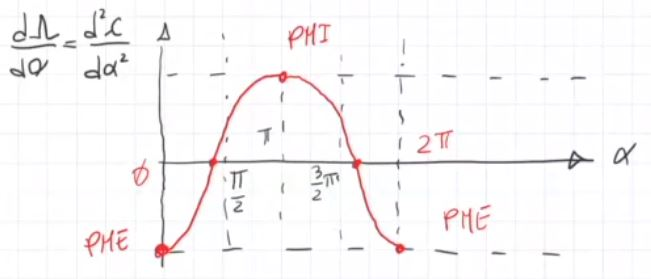
\includegraphics[height=3cm]{../lezione5/img5.JPG}
\end{center}
